\documentclass[14pt]{extbook}
\usepackage{multicol, enumerate, enumitem, hyperref, color, soul, setspace, parskip, fancyhdr} %General Packages
\usepackage{amssymb, amsthm, amsmath, bbm, latexsym, units, mathtools} %Math Packages
\everymath{\displaystyle} %All math in Display Style
% Packages with additional options
\usepackage[headsep=0.5cm,headheight=12pt, left=1 in,right= 1 in,top= 1 in,bottom= 1 in]{geometry}
\usepackage[usenames,dvipsnames]{xcolor}
\usepackage{dashrule}  % Package to use the command below to create lines between items
\newcommand{\litem}[1]{\item#1\hspace*{-1cm}\rule{\textwidth}{0.4pt}}
\pagestyle{fancy}
\lhead{Progress Quiz 4}
\chead{}
\rhead{Version A}
\lfoot{9187-5854}
\cfoot{}
\rfoot{Spring 2021}
\begin{document}

\begin{enumerate}
\litem{
Solve the radical equation below. Then, choose the interval(s) that the solution(s) belongs to.\[ \sqrt{21 x^2 - 63} - \sqrt{-42 x} = 0 \]\begin{enumerate}[label=\Alph*.]
\item \( \text{All solutions lead to invalid or complex values in the equation.} \)
\item \( x_1 \in [-4, -1] \text{ and } x_2 \in [-1,2] \)
\item \( x \in [0,2] \)
\item \( x \in [-4,-1] \)
\item \( x_1 \in [0, 2] \text{ and } x_2 \in [3,4] \)

\end{enumerate} }
\litem{
Solve the radical equation below. Then, choose the interval(s) that the solution(s) belongs to.\[ \sqrt{-56 x^2 + 16} - \sqrt{-4 x} = 0 \]\begin{enumerate}[label=\Alph*.]
\item \( x \in [-0.57,-0.43] \)
\item \( x \in [0.56,0.67] \)
\item \( \text{All solutions lead to invalid or complex values in the equation.} \)
\item \( x_1 \in [-0.57, -0.43] \text{ and } x_2 \in [-3.43,2.57] \)
\item \( x_1 \in [0.49, 0.56] \text{ and } x_2 \in [-3.43,2.57] \)

\end{enumerate} }
\litem{
Choose the graph of the equation below.\[ f(x) = - \sqrt[3]{x - 14} + 7 \]\begin{enumerate}[label=\Alph*.]
\begin{multicols}{2}\item 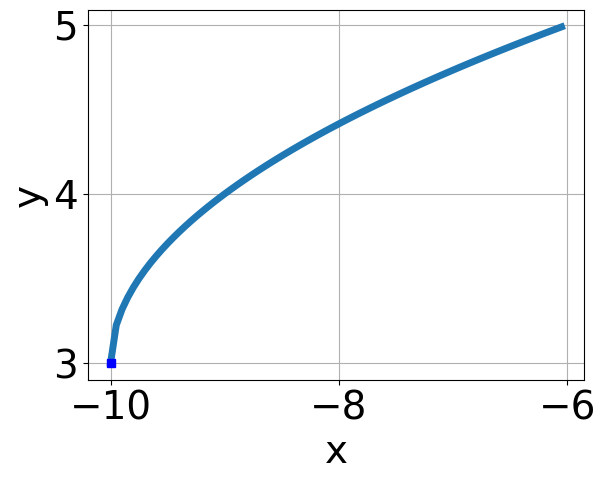
\includegraphics[width = 0.3\textwidth]{../Figures/radicalEquationToGraphAA.png}\item 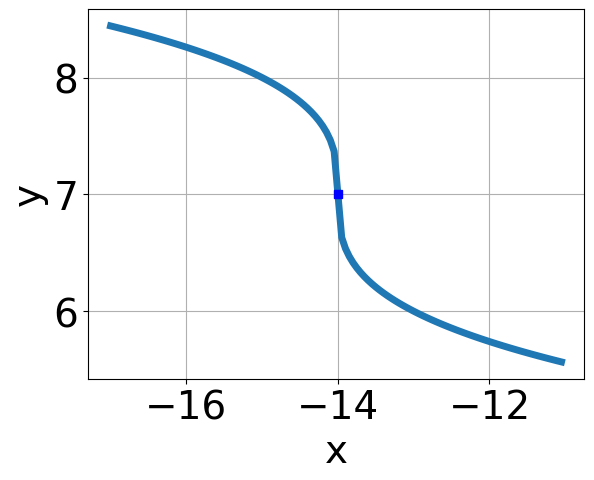
\includegraphics[width = 0.3\textwidth]{../Figures/radicalEquationToGraphBA.png}\item 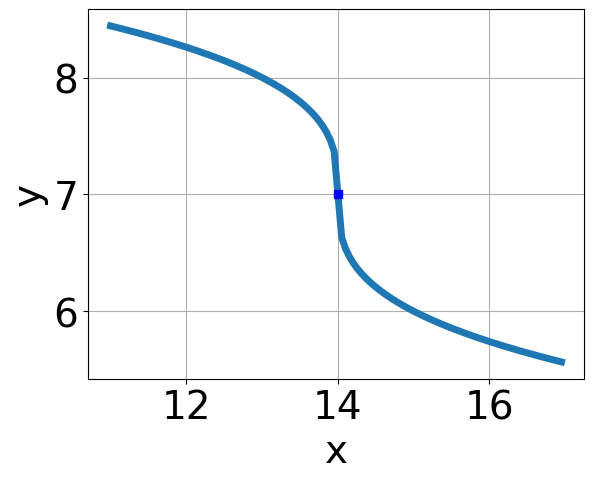
\includegraphics[width = 0.3\textwidth]{../Figures/radicalEquationToGraphCA.png}\item 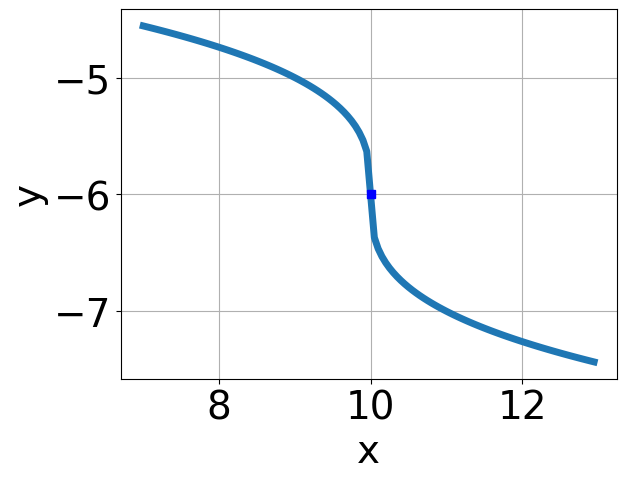
\includegraphics[width = 0.3\textwidth]{../Figures/radicalEquationToGraphDA.png}\end{multicols}\item None of the above.
\end{enumerate} }
\litem{
What is the domain of the function below?\[ f(x) = \sqrt[6]{8 x + 5} \]\begin{enumerate}[label=\Alph*.]
\item \( (-\infty, a], \text{where } a \in [-0.65, -0.34] \)
\item \( [a, \infty), \text{ where } a \in [-0.68, -0.23] \)
\item \( [a, \infty), \text{where } a \in [-1.75, -1.34] \)
\item \( (-\infty, \infty) \)
\item \( (-\infty, a], \text{where } a \in [-2.11, -1.44] \)

\end{enumerate} }
\litem{
Choose the equation of the function graphed below.
\begin{center}
    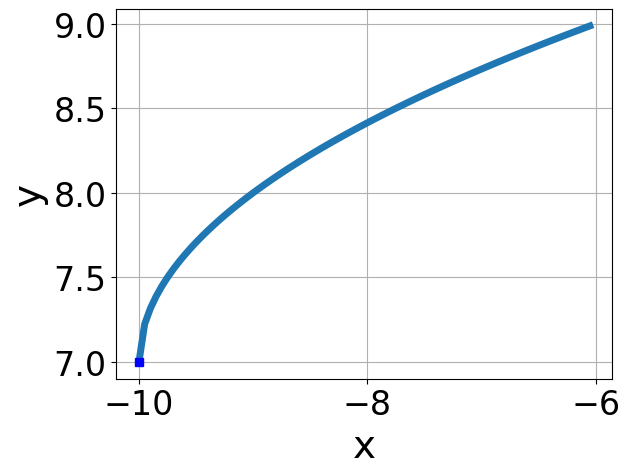
\includegraphics[width=0.5\textwidth]{../Figures/radicalGraphToEquationCopyA.png}
\end{center}
\begin{enumerate}[label=\Alph*.]
\item \( f(x) = - \sqrt{x + 8} + 3 \)
\item \( f(x) = \sqrt{x + 8} + 3 \)
\item \( f(x) = \sqrt{x - 8} + 3 \)
\item \( f(x) = - \sqrt{x - 8} + 3 \)
\item \( \text{None of the above} \)

\end{enumerate} }
\litem{
What is the domain of the function below?\[ f(x) = \sqrt[7]{3 x - 5} \]\begin{enumerate}[label=\Alph*.]
\item \( \text{The domain is } [a, \infty), \text{   where } a \in [0.9, 3.5] \)
\item \( (-\infty, \infty) \)
\item \( \text{The domain is } [a, \infty), \text{   where } a \in [-0.7, 0.9] \)
\item \( \text{The domain is } (-\infty, a], \text{   where } a \in [1.1, 4.6] \)
\item \( \text{The domain is } (-\infty, a], \text{   where } a \in [0.5, 1.3] \)

\end{enumerate} }
\litem{
Choose the equation of the function graphed below.
\begin{center}
    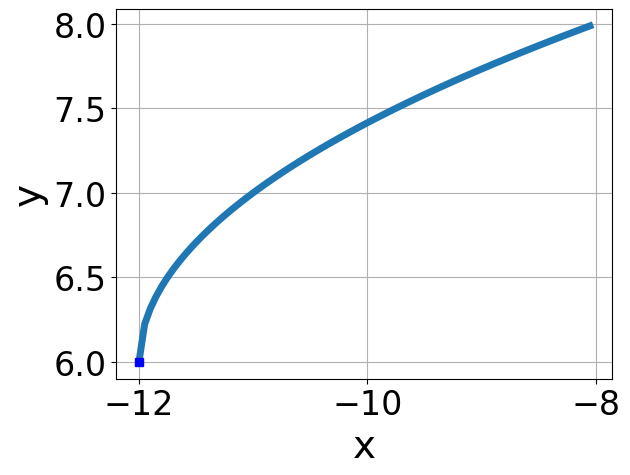
\includegraphics[width=0.5\textwidth]{../Figures/radicalGraphToEquationA.png}
\end{center}
\begin{enumerate}[label=\Alph*.]
\item \( f(x) = - \sqrt[3]{x + 12} + 6 \)
\item \( f(x) = - \sqrt[3]{x - 12} + 6 \)
\item \( f(x) = \sqrt[3]{x + 12} + 6 \)
\item \( f(x) = \sqrt[3]{x - 12} + 6 \)
\item \( \text{None of the above} \)

\end{enumerate} }
\litem{
Choose the graph of the equation below.\[ f(x) = - \sqrt{x - 8} - 6 \]\begin{enumerate}[label=\Alph*.]
\begin{multicols}{2}\item 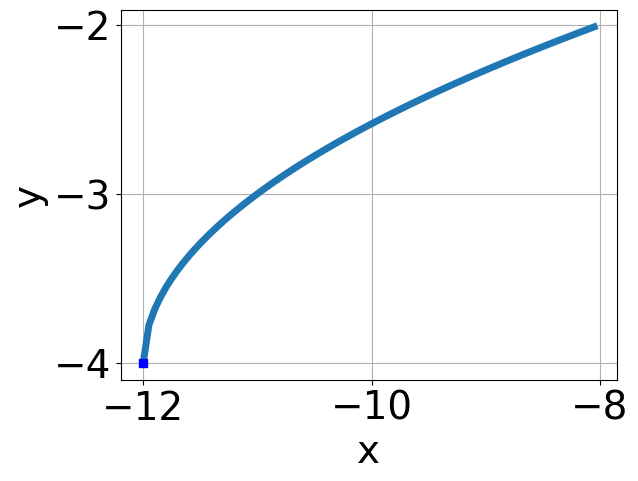
\includegraphics[width = 0.3\textwidth]{../Figures/radicalEquationToGraphCopyAA.png}\item 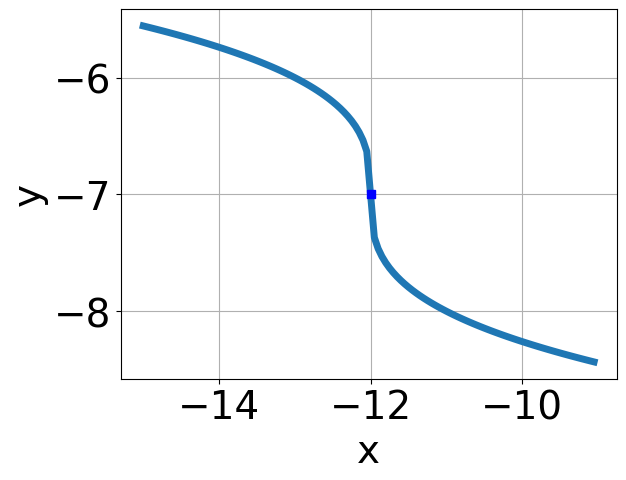
\includegraphics[width = 0.3\textwidth]{../Figures/radicalEquationToGraphCopyBA.png}\item 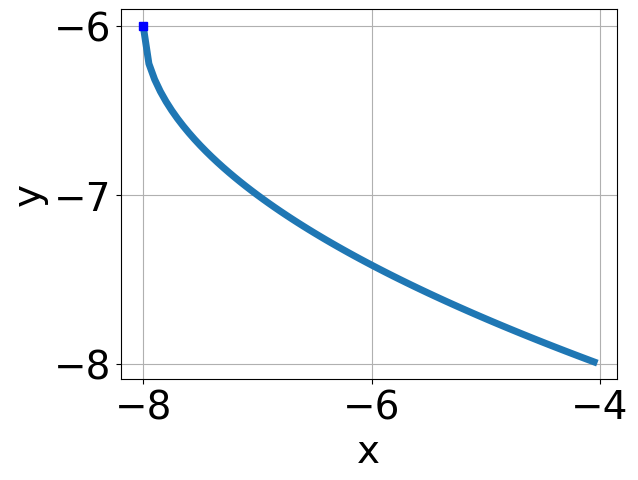
\includegraphics[width = 0.3\textwidth]{../Figures/radicalEquationToGraphCopyCA.png}\item 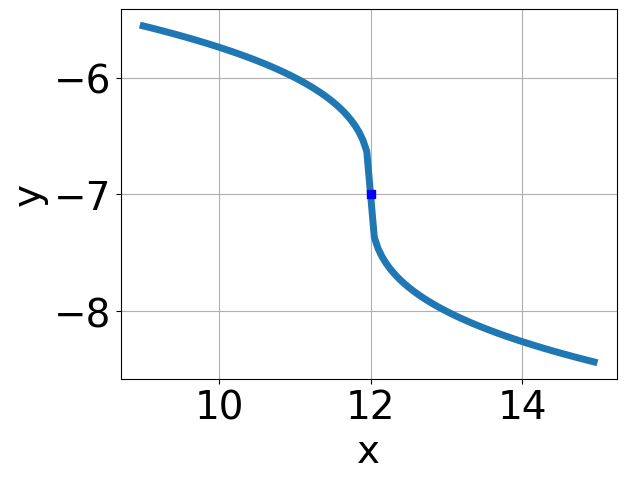
\includegraphics[width = 0.3\textwidth]{../Figures/radicalEquationToGraphCopyDA.png}\end{multicols}\item None of the above.
\end{enumerate} }
\litem{
Solve the radical equation below. Then, choose the interval(s) that the solution(s) belongs to.\[ \sqrt{-8 x - 9} - \sqrt{6 x - 9} = 0 \]\begin{enumerate}[label=\Alph*.]
\item \( x \in [-1.36,-1.25] \)
\item \( x \in [-0.1,0.1] \)
\item \( \text{All solutions lead to invalid or complex values in the equation.} \)
\item \( x_1 \in [-1.23, -0.85] \text{ and } x_2 \in [-1,1] \)
\item \( x_1 \in [-1.23, -0.85] \text{ and } x_2 \in [1.5,3.5] \)

\end{enumerate} }
\litem{
Solve the radical equation below. Then, choose the interval(s) that the solution(s) belongs to.\[ \sqrt{-8 x - 7} - \sqrt{8 x - 9} = 0 \]\begin{enumerate}[label=\Alph*.]
\item \( x_1 \in [-0.95, -0.84] \text{ and } x_2 \in [-0.09,0.28] \)
\item \( x \in [0.04,0.3] \)
\item \( \text{All solutions lead to invalid or complex values in the equation.} \)
\item \( x \in [-1.03,-0.99] \)
\item \( x_1 \in [-0.95, -0.84] \text{ and } x_2 \in [0.85,2.01] \)

\end{enumerate} }
\end{enumerate}

\end{document}